\large
%%ANC headphones are becoming widely used in consumer electronics, however often the attenuation decreases rapidly with an increased frequency. 
%%This is due to the delays introduced by sampling and reconstructing the signals.
%This can be due to delay in the ANC system. 
%A Linear Prediction (LP) algorithm is proposed to predict $P$ samples, corresponding to the system delay, to compensate for the delay.   
%\begin{centering}
%	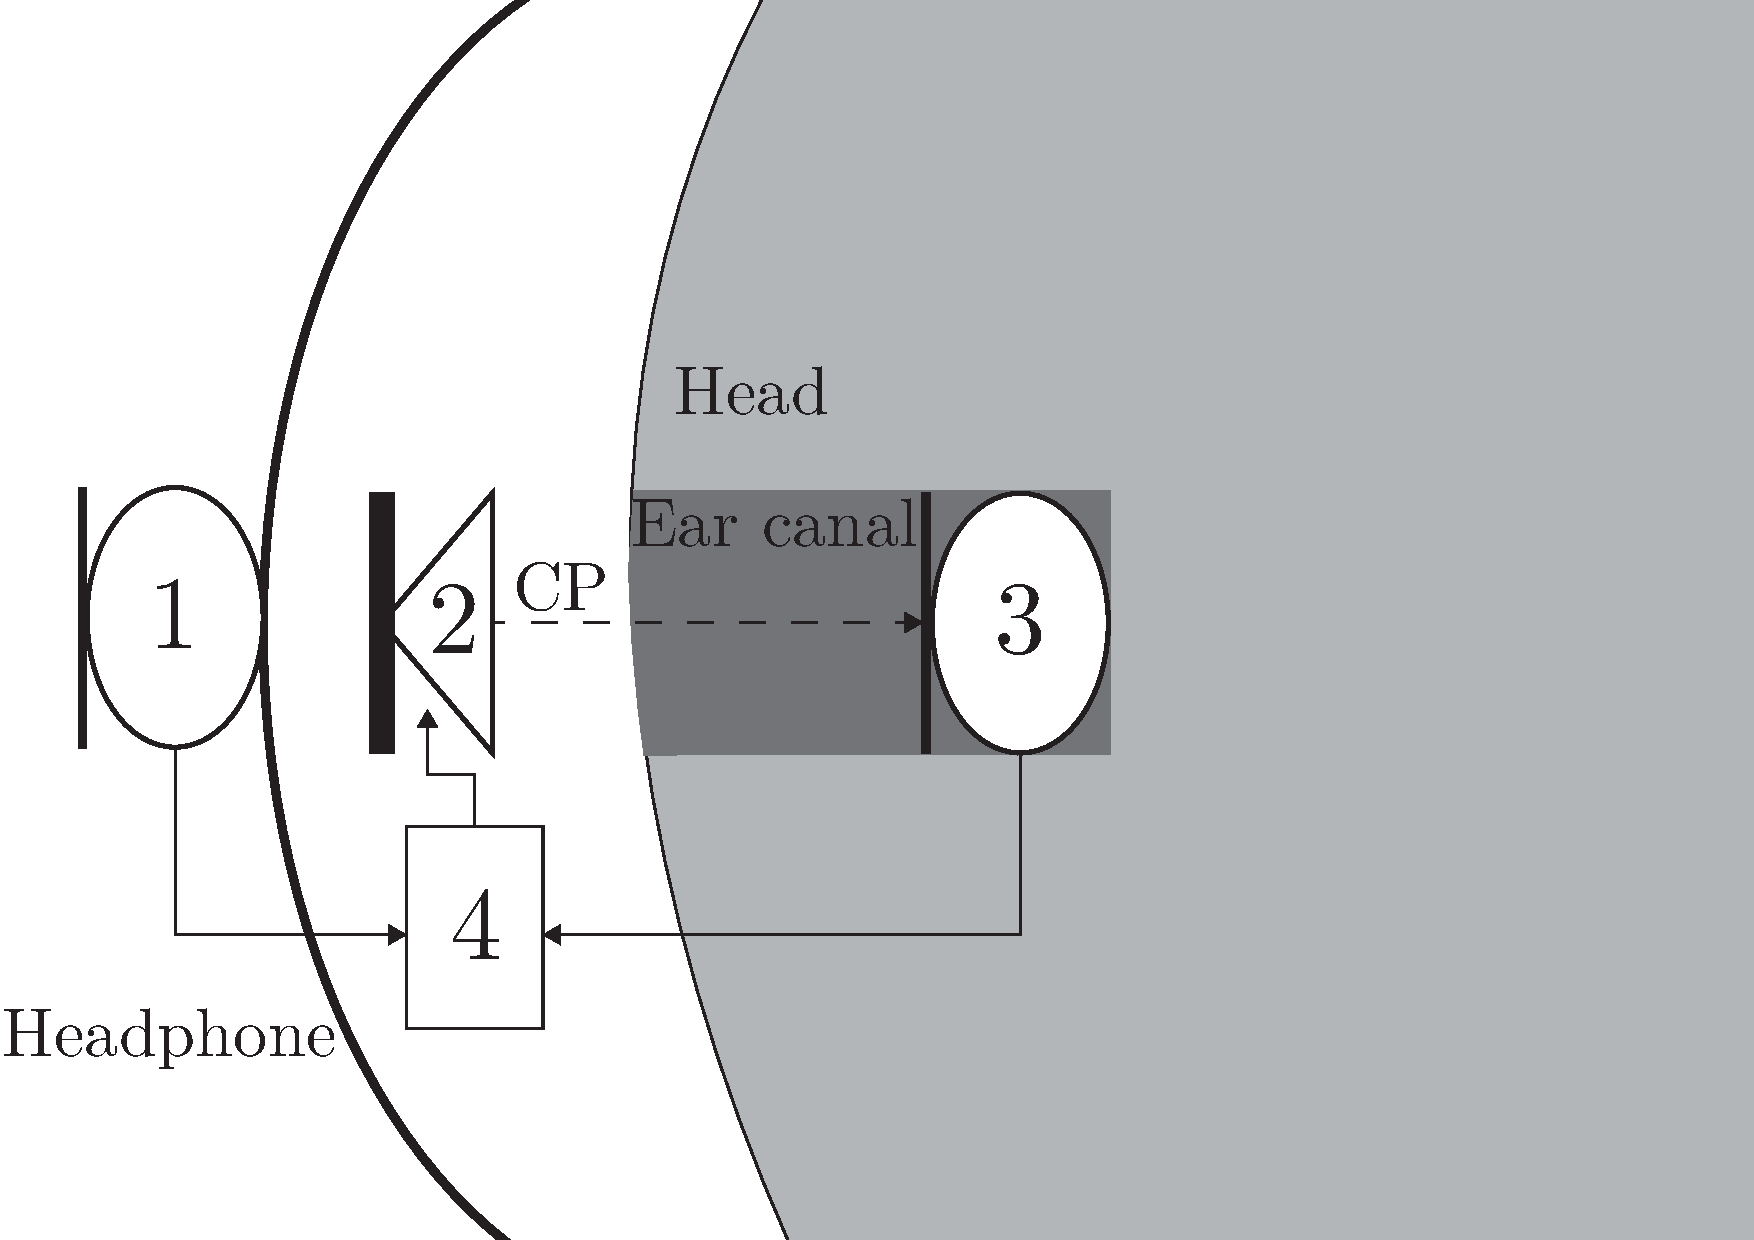
\includegraphics[width=\textwidth]{figures/BasicOverviewZoomed.pdf}
%\end{centering}
%The simulated test setup consists of a reference microphone (1), a headphone speaker (2), an error microphone (3) and a DSP (4). %The delays are introduced by sampling the microphones and playing the counterphase signal through the loudspeaker.\\ 

%
%
%
%%Oliver Edition
%% % ANC headphones are becoming increasingly popular, especially for canceling speech. 
% In order to cancel speech, a feedforward solution is proposed.
% However this method introduces increasingly large delay, and to accommodate this problem, a Linear Prediction (LP) algorithm is proposed to predict $P$ samples
% of the speech signal, thus compensating for the delay.
%
%
%\begin{centering}
%	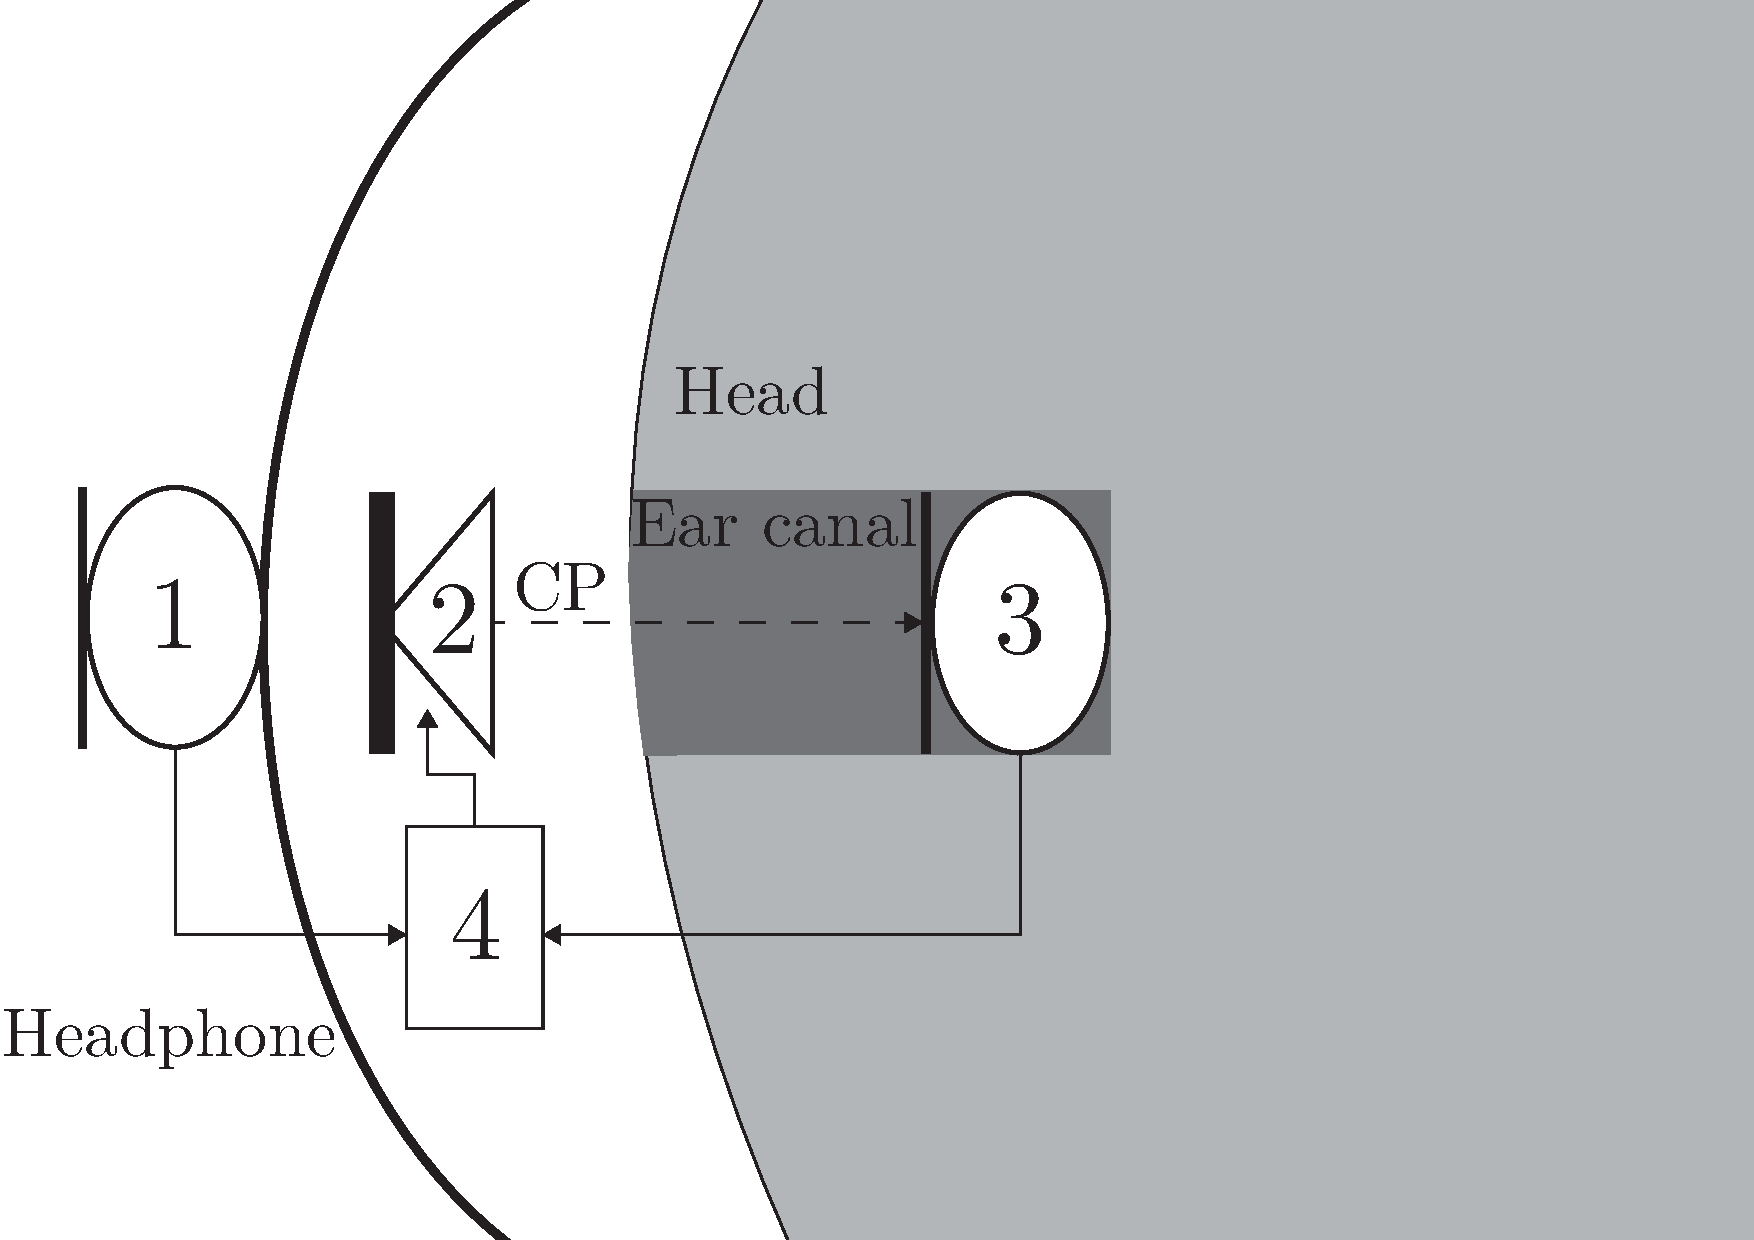
\includegraphics[width=\textwidth]{figures/BasicOverviewZoomed.pdf}
%\end{centering}
%The simulated test setup consists of a reference microphone (1), a headphone speaker (2), an error microphone (3) and a DSP (4). 
%
%speech
%feedforward
%delay
%LP


%ANC headphones are used to attenuate various noise sources, among these are speech.


ANC headphones lack the ability to attenuate speech.
In order accommodate this problem, a feedforward system is necessary.
This topology introduces delay, which decreases the attenuation of the system.
In order to cope with this delay, a Linear Prediction (LP) scheme is proposed.


 











